
\chapter{Methods}
\section{Toric Code and Syndrome Measurements}
\subsection{Qubit layout and operators}
	The Toric code exists on a L by L lattice, consisting of $2L^2$ physical qubits. Ths lattice has periodic boundary conditions. For every row of the lattice there are 2 qubits at every site; forming a grid and a cogrid. The arrangements of the grid allows for plaquette operators to exist at every (i,j) site on the grid. Every plaquette operator is bordered by 4 qubits.
	
	Each qubit on the grid can take the value of -1 or 1, and its value is stored in a L by 2 by L array ($Q(L,2,L)$), to store the information about the grid and cogrid qubits. 
	
	Plaquette operators are stored in a L by L array ($S(L,L)$), and can also take the value of -1 or 1. 
	
	All qubits on the torus are initialized to to an error free state represented by `1'. When a physical qubit on the torus experiences an error, it's value is changed to `-1'. 
	
	 The syndrome of the code is determined through measuring all of the plaquette operators. A measurement of a plaquette opertor corresponds to;
	 \begin{equation}
		P_{i,j}=Z_{left} \otimes Z_{right} \otimes Z_{above} \otimes Z_{below} 
		\label{eq:plaquette]}
	 \end{equation}
	Equation \ref{eq:plaquette]} states that the value of plaquette i is equal to the measurement a Z operator on each neighbouring qubit. This corresponds to each value $P_i$ in the L by L plaquette array equalling the multiplication of the values of the surrounding qubits. i.e. multiply together the values of the qubits located at left, right, above and below the stabilizer. 
	\begin{equation}
		S(i,j) = 	Q(i,0,j)\cross Q(i,1,j)\cross Q(i+1,0,j+1) \cross Q(i+1,1,j+1)
	\end{equation}
	
	The measurements of the stabilizers creates an array called the syndrome, which consists of the locations of all the anyon locations,represented by -1's. 
	
	The syndrome measurement reveals information about the error locations on the torus. 
	A successful correction operation on the toric code must return the codespace to its ground state. The ground state of the toric code is degenerate, and is formed from the stabilizer space of the code. That is, any state which can be formed from a product of stabilzers, is a ground state of the code. The ground state of the toric code is populated by homologically trivial loops of -1's on the grid. A correction scheme on the toric code would aim to match any errant pairs of -1's in the stabilizer array (which indicate the end points of error chains), in an attempt to forms error-loops which are trivial, and return the code to its ground state.
	
	After applying these flips, the homology class of the code is determined by measuring a two test line of operators across the code in conjugate directions. If the eigenvalue of one of these measurements is -1, then there exists a nontrivial cycle, and the qubit representing that direction failed to be recovered from error. 
	\section{Uncorrelated Errors}
	Two error models were implemented. Firstly, an uncorrelated error model was used to validate the function of the code. The results from this uncorrelated error model was compared to \cite{Stace2010} for confirmation. 

	The uncorrelated error model was implemented by looping over every element in the qubit array, and flipping a qubits state with probability $p$. 
	The optimal decoding solution for this error model is to match anyons with least weight. A matrix of distances between anyons can be generated and passed to an implementation of Edmonds perfect matching. Kolmogorov's BlossomV code \cite{Kolmogorov2009} is a suitable implementation of this least-weight perfect-matching algorithm. This uncorrelated error model is analogous to noise on the qubits.

	\section{Correlated Errors}
	Random walks were used to simulated correlated errors on the toric code. 
	A random point on $Q$ was chosen as the starting point for the random walk. From this position, errors were designed to walk diagonally around the grid. Due to the offset nature of Q, diagonal movements are the shortest distance movements that anyons can make around the grid, and are therefore most likely. The walker was allowed to evolve for $N$ steps (the correlation length), with each movement direction being equally likely. 
	All locations that the walker moved to were then flipped.
	
	\section{Improved Decoders}
	Two new decoders are proposed to reduce the failure rate of correlated errors. Random walks have been shown to have expected Manhattan walk lengths \ref{eq:manahat_expected}. We postulate increasing the chance of matchings near this expected length should decrease the failure rate of the code. 
	
	We will heuristically investigate the effect of concatenating the least weight perfect matching procedure of the naive decoder with a reduction in weight around various distances.
	
	The improved decoders present make use of the same BlossomV matching algorithm of the least weight decoder. The new decoder add preference to selecting matches at new locations, but reducing the `perceived distance' that the blossomV code passes. Thus, to increase the weight of a pair for matching, the adjusted distance is reduced from the original Manhattan distance. 
	\subsection{Gaussian Decoder}
	
	The first method of optimizing for correlated errors, is to use a gaussian correction to offset the effect of correlating the errors. The optimal gaussian to reduce the failure rate of the code can be found by varying the parameters of the gaussian. To do so, the center of the gaussian is swept through [0,N] and the variance of the gaussian is swept though(0,$\sigma_{max}$]. The strength of the gaussian correction is held constant to reduce the computational overhead. The naive decoder has been proven to yield the lowest error rates when error is uncorrelated. For uncorrelated errors, the most common chain length is 0. A heuristic argument can be made that if the walk is not most likely to be at 0 (as is the case for correlated errors \ref{fig:exactpdfs}), then there is no reason to preference this length of walk over other lengths (for example, the expected walk length). 
	\\\\
	The gaussian correction reduces the Manhattan distance of anyons near the centre of the gaussian ($\overline{w}$).  It does so by creating a gaussain centred at $\overline{w}$, with variance $\sigma^2$; and then inverting it, and shifting it up by unity. 
	\begin{align}
	A &= M \left( 1 - e^{\frac{-(M-\overline{w})^2}{2\cdot \sigma^2}} \right) 
	\label{eq:gaussainadjust}
	\end{align}
	Equation \ref{eq:gaussainadjust} shows how the adjustment works. In equation \ref{eq:gaussainadjust} $A$ represents the adjusted value, $M$ is the original Manhattan distance, $\overline{w}$ is the centre of the gaussain, and $\sigma^2$ is the variance or width of the gaussain.
	The behaviour of this decoder is shown in figure \ref{fig:gaussiancorrection}. The expected walk length of a N=32 walk is 5.016; figure \ref{fig:gaussiancorrection} is typical of a gaussian that is closely `centred' at this expected walk length.
	\begin{figure}
		\centering
		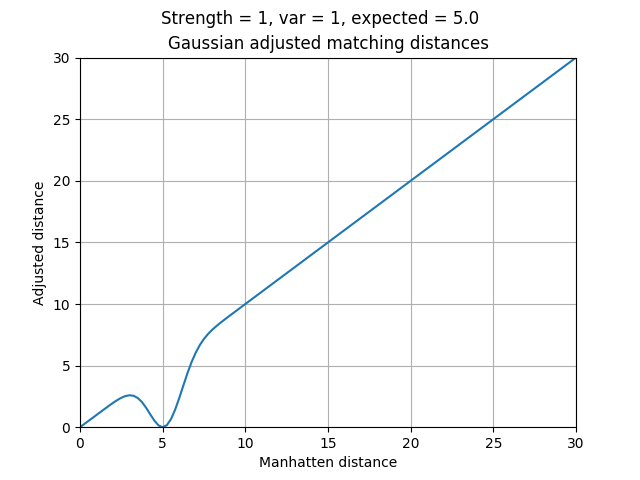
\includegraphics[width = 0.7\textwidth]{figs/gaussian-20.png}
		\caption{The behaviour of the Gaussian decoder. The decoder reduces the adjusted distance near a chosen Manhattan distance.}
		\label{fig:gaussiancorrection}
	\end{figure}
	\subsection{Manhattan PDF Decoder}
	